\section{Bil} \label{sec:bil}

\subsection{DistanceSensor}
%%%%%%%%%%%%%%%%%%%%%%%%%%%%%%%%%%%%%%%%%%%%%%%%%%%%%%%%%%%%%%%%%
%																%
%      ++++++++++++ Design af Afstandssensor ++++++++++++++		%
%																%
%%%%%%%%%%%%%%%%%%%%%%%%%%%%%%%%%%%%%%%%%%%%%%%%%%%%%%%%%%%%%%%%%

Afstandssensorene leveres formonteret på chip hvor benene fra IC'en er trukket til harwinpins som let kan tilgås. Der benyttes I2C-protokol til kommunikation med Pi'en. Ved kommunikation benyttes følgende pins: 

\begin{itemize}
	\item pin 1: Temporary Default
	\item pin 2: Address Announce / Status
	\item pin 3: Benyttes ikke
	\item pin 4: SDA: Data
	\item pin 5: SCL: Clock
	\item pin 6: GND: Reference
	\item pin 7: VCC: Forsyning
\end{itemize}

\noindent
\textit{SDA}-linjen kommunikerer data ud med reference til GND.
\noindent
\textit{SCL}-linjen sørger for at holde timing. 
\noindent
\textit{AA/Status} benyttes til at angive om sensoren er i gang med at foretage en range- reading. Status-pin'en holdes højt så længe sensoren scanner, og trækkes lavt når operationen er fuldført. Dette angiver at data er klar til levering. Når status-pin'en er høj ignoreres al I2C-kommunikation, således at sensoren kan arbejde uforstyrret. 
\noindent
\textit{Temp-adresse}-pin'en benyttes til at initiere sensoren med en ønsket adresse, denne pin sætte høj ved power-up, kan en brugerdefineret adresse sendes til sensoren, i dette tilfælde benyttes unikke 8-bit adresser til sensorerne.

Herefter skrives en klasse \texttt{distanceSensor} der kan håndtere de ønskede kald til de 4 afstandssensorer. 
Denne klasse skal indeholde funktion til at tilgå sensorerne. Klassen initieres med constructoren hvori der åbne for I2C-devicet, samt at der sætte den foromtalte adresse. Detudover skal klassen indeholde metoden: \texttt{getDistance()}, i denne funktion foretages et read-kald med den pågældende sensors adresse. 
Følgende kommander benyttes for at kommunikere med en med en given adresse: 











\clearpage

\subsection{Klassediagram}
I dette afsnit beskrives det overordnede design på den software der kommer til at ligge på Pi. På figur \ref{fig:cd_pi} ses et klassediagram der opdeler funktionaliteten i klasser.

\begin{figure}[h]
\centering
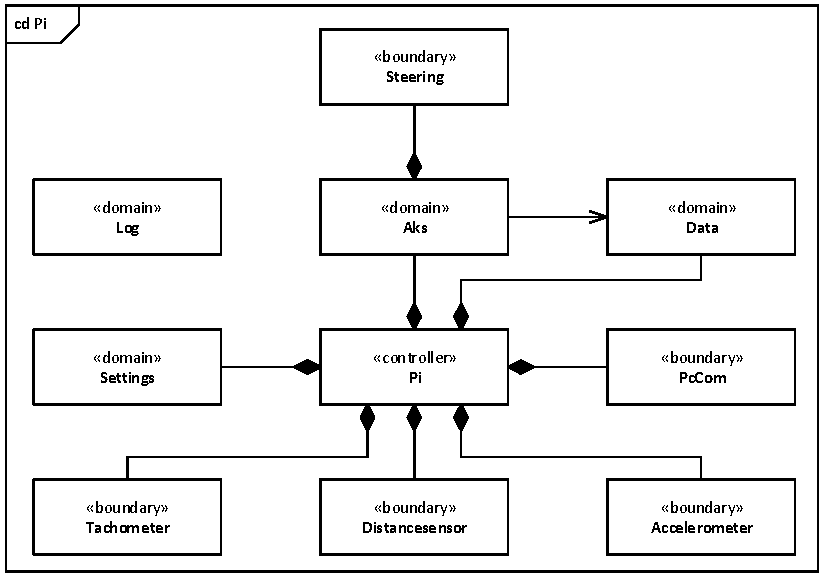
\includegraphics[width=\textwidth* 9/10]{../fig/diagrammer/bil/cd_pi.pdf}
\caption{Klasse diagram over Pi}
\label{fig:cd_pi}
\end{figure}

\subsubsection{Controller-klasse: Pi}
Controller-klassen Pi indeholder main funktionen og har derfor ansvaret for at styre slagets gang. Klassen skal derfor iværksætte initialisering af alle de klasser som den har ejerskab over. En af klassen ansvarsområder er at indsamle data fra sensorerne, og dette gøres ved at starte en særskilt tråd til dette. Denne tråd skal også sørge for at iværksætte Aks-klassen hver gang nye data er indsamlet.

\subsubsection{Domain-klasse: Aks}
Domain-klassen analyserer indkomne sensordata og i tilfælde at bilen er ved at køre ind i en forhindring, blokeres brugerinput og der styres udenom eller bremses.

\subsubsection{Domain-klasse: Data}
Denne klasse har til formål at indsamle alle sensordata i en datastruktur. Disse data gemmes i memory kan ikke overstige en defineret størrelse. Brugerinput gemmes ikke i denne klasse.

\subsubsection{Domain-klasse: Log}
Denne klasse har til formål at gemme samtlige systemhændelser i den fil, så kilden til eventuelle programcrash kan identificeres. Alle klasser på Pi har en reference til denne log, så de hver i sær kan skrive til den. På figur \ref{fig:cd_pi} er der undladt at lave pile fra alle klasser til denne, da dette vil gøre diagrammet uoverskueligt. 

\subsubsection{Domain-klasse: Settings}
Settings er datastruktur der indeholder indstillinger for maksimal hastighed, AKS status, og styretøjs kalibrering. Indstillingerne er gemt i en fil som kan tilgås af Pi-klassen og Steering-klassen.

\subsubsection{Boundary-klasse: PcCom}
Boundary-klassen PcCom håndterer kommunikationen imellem PC og Bil. Denne kommunikation sker vha. UDP via Wi-Fi.

\subsubsection{Boundary-klasse: Steering}
I denne klasse styres bilens aktautorer. Dette er altså en driver til både motoren der skaber fremdrift og servo-motoren der styrer forhjulene. Klassen tager ligeledes højde for brugers indstillinger.

\subsubsection{Boundary-klasse: Tachometer}
Denne klasse håndterer kommunikationen til bilens tachometer og konverterer sensordata til brugbar hastighedsmåling.

\subsubsection{Boundary-klasse: DistanceSensor}
Denne klasse håndterer kommunikationen til bilens afstandssensorer og konverterer sensordata til brugbar distancemålinger. Klassen håndterer alle fire sensorer.

\subsubsection{Boundary-klasse: Accelerometer}
Denne klasse håndterer kommunikationen til bilens accelerometer og konverterer sensordata til brugbar g-måling.

\clearpage

\subsection{Sekvensdiagrammer}
Herunder er udarbejdet sekvensdiagrammer for den funktionalitet som Pi blokken på bilen skal have. Der er tage udgangspunkt i de de tidligere fremstillede use cases. Sekvensdiagrammer for UC8 og UC12 er udeladt, da disse kun indeholder handlinger over interaktion imellem bruger og PC.

\begin{figure}[h]
\centering
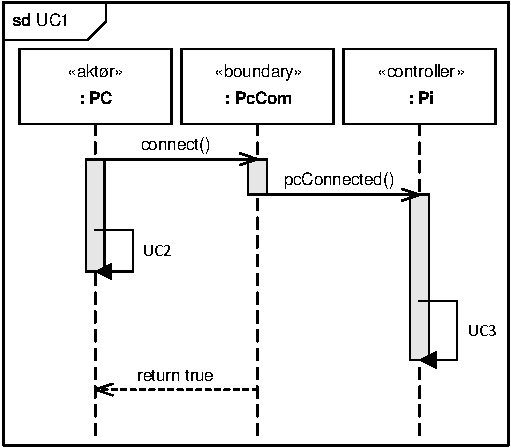
\includegraphics[]{../fig/diagrammer/bil/sd_uc1.pdf}
\caption{Sekvensdiagram over  bilens funktionalitet i UC1: Aktiver system}
\label{fig:sd_uc1_bil}
\end{figure}

\begin{figure}[h]
\centering
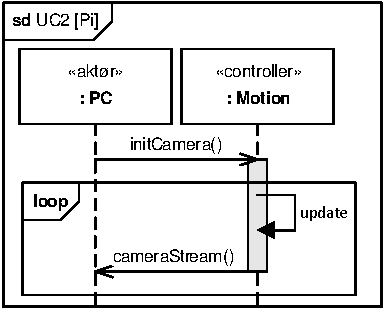
\includegraphics[]{../fig/diagrammer/bil/sd_uc2.pdf}
\caption{Sekvensdiagram over  bilens funktionalitet i UC2: Stream video}
\label{fig:sd_uc2_bil}
\end{figure}

\begin{landscape}

\begin{figure}[h]
\centering
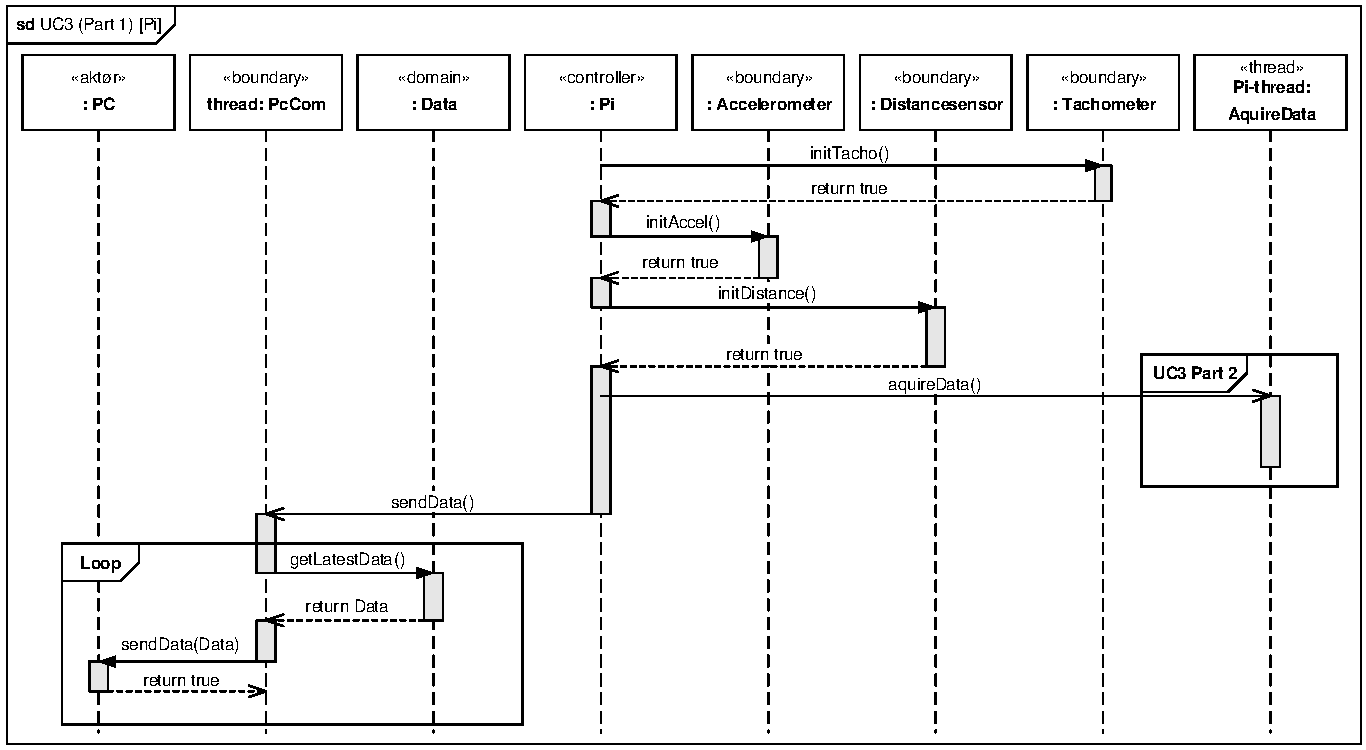
\includegraphics[]{../fig/diagrammer/bil/sd_uc3_1.pdf}
\caption{Sekvensdiagram over  bilens funktionalitet i UC3: Overvåg sensorer - Del 1}
\label{fig:sd_uc3_1_bil}
\end{figure}

\begin{figure}[h]
\centering
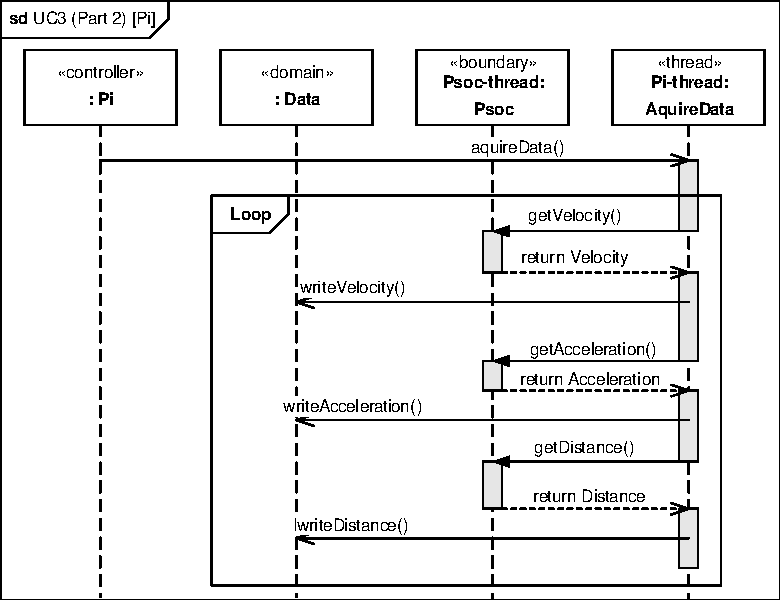
\includegraphics[]{../fig/diagrammer/bil/sd_uc3_2.pdf}
\caption{Sekvensdiagram over  bilens funktionalitet i UC3: Overvåg sensorer - Del 2}
\label{fig:sd_uc3_2_bil}
\end{figure}

\end{landscape}

\begin{figure}[h]
\centering
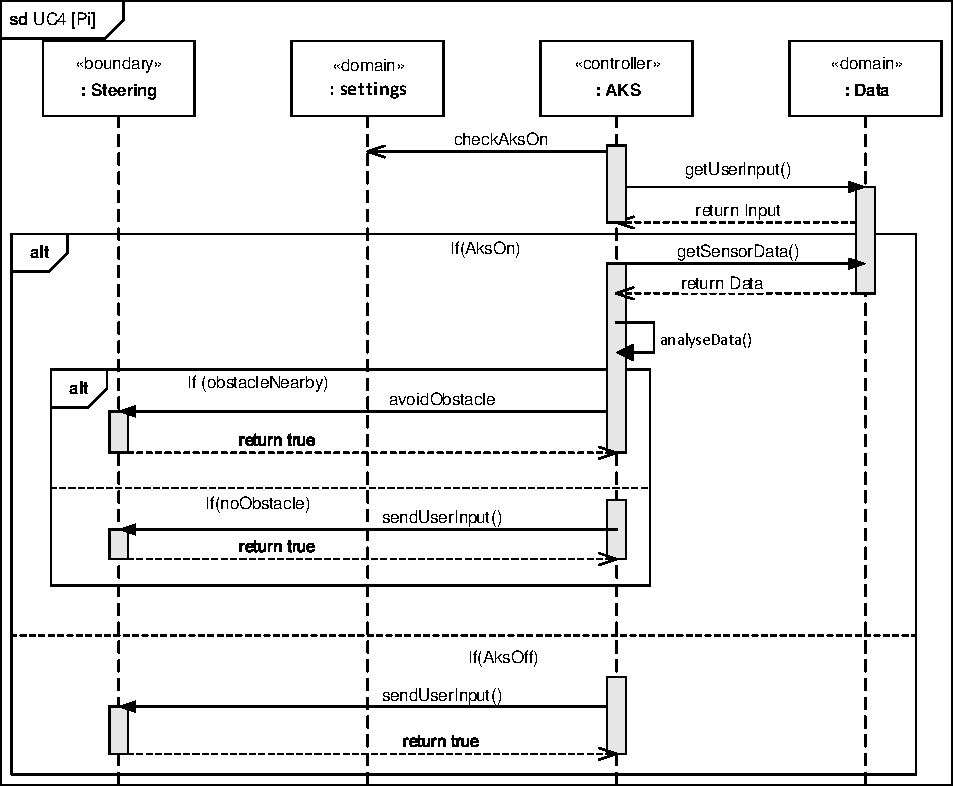
\includegraphics[]{../fig/diagrammer/bil/sd_uc4.pdf}
\caption{Sekvensdiagram over  bilens funktionalitet i UC4: Undvig forhindring}
\label{fig:sd_uc4_bil}
\end{figure}

\begin{figure}[h]
\centering
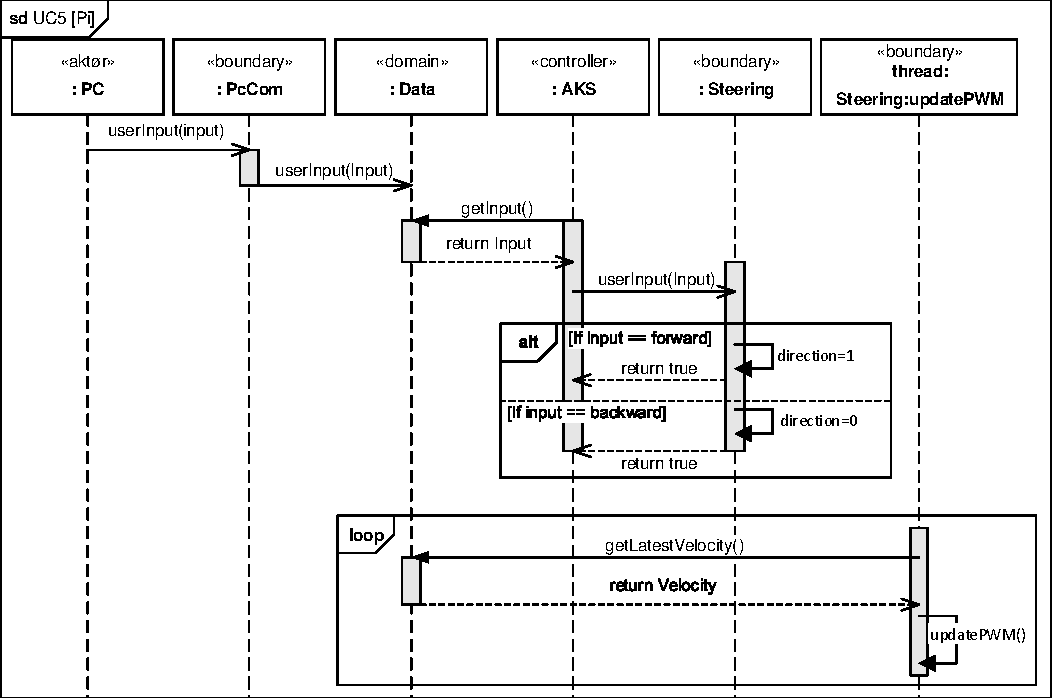
\includegraphics[]{../fig/diagrammer/bil/sd_uc5.pdf}
\caption{Sekvensdiagram over  bilens funktionalitet i UC5: Kør bil frem/tilbage}
\label{fig:sd_uc5_bil}
\end{figure}

\begin{figure}[h]
\centering
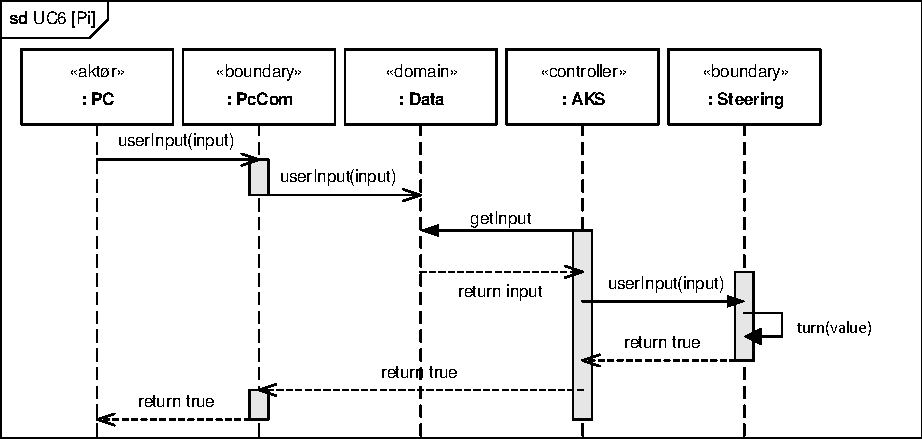
\includegraphics[]{../fig/diagrammer/bil/sd_uc6.pdf}
\caption{Sekvensdiagram over  bilens funktionalitet i UC6: Drej til højre/venstre}
\label{fig:sd_uc6_bil}
\end{figure}

\begin{figure}[h]
\centering
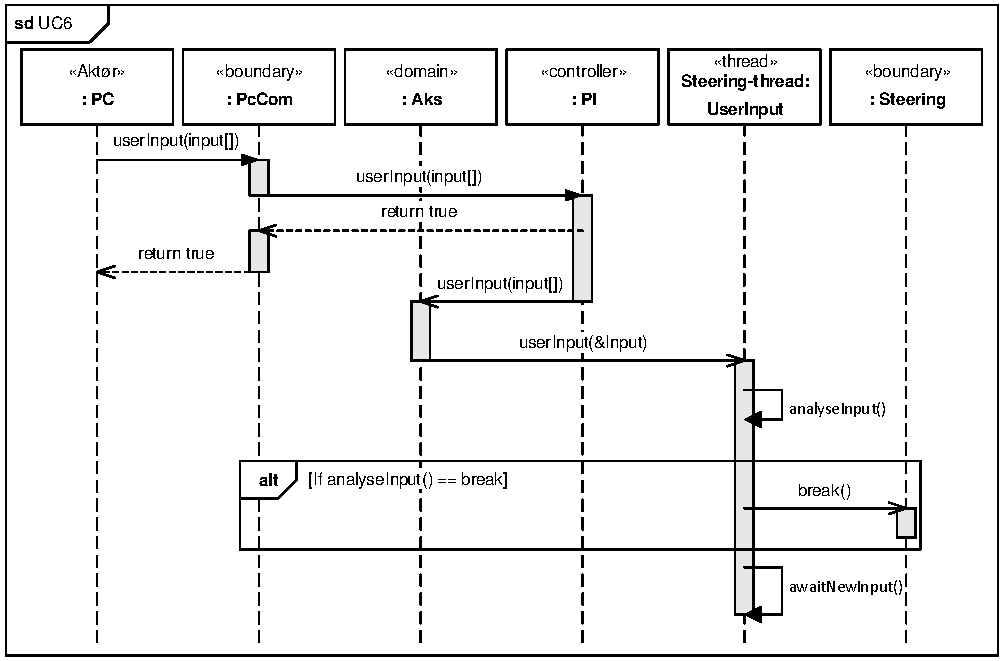
\includegraphics[]{../fig/diagrammer/bil/sd_uc7.pdf}
\caption{Sekvensdiagram over  bilens funktionalitet i UC7: Brems bil}
\label{fig:sd_uc7_bil}
\end{figure}

\begin{figure}[h]
\centering
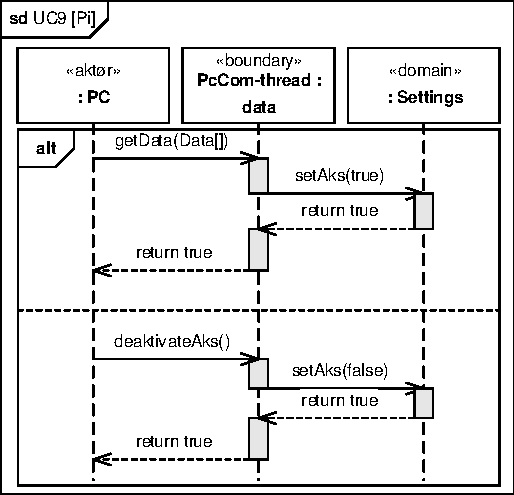
\includegraphics[]{../fig/diagrammer/bil/sd_uc9.pdf}
\caption{Sekvensdiagram over  bilens funktionalitet i UC9: Tænd/sluk AKS}
\label{fig:sd_uc9_bil}
\end{figure}

\begin{figure}[h]
\centering
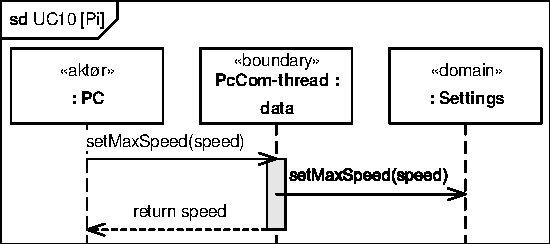
\includegraphics[]{../fig/diagrammer/bil/sd_uc10.pdf}
\caption{Sekvensdiagram over  bilens funktionalitet i UC10: Indstil makshastighed}
\label{fig:sd_uc10_bil}
\end{figure}

\begin{figure}[h]
\centering
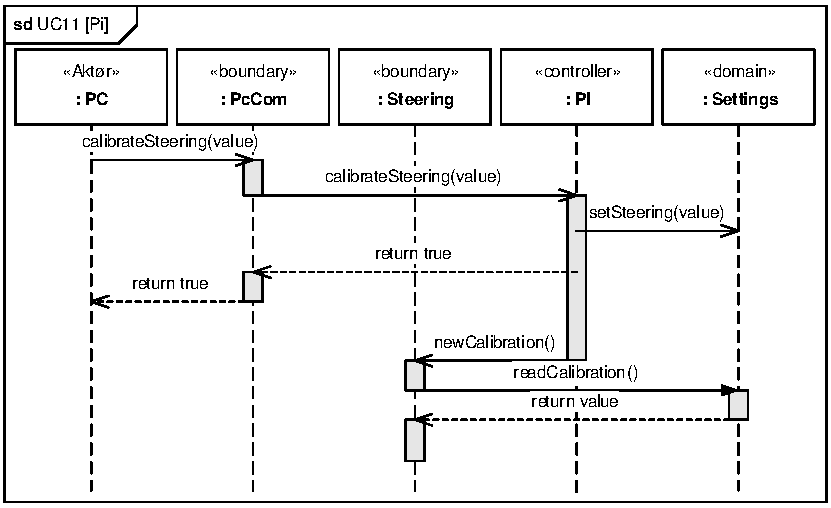
\includegraphics[]{../fig/diagrammer/bil/sd_uc11.pdf}
\caption{Sekvensdiagram over  bilens funktionalitet i UC11: Kalibrer styretøj}
\label{fig:sd_uc11_bil}
\end{figure}

\clearpage
\subsection{Klassebeskrivelser}
% ++++++++++++ Controller PSoC Master klassen ++++++++++++++
\subsubsection{Boundary-klasse: DistanceSensor}

\begin{figure}[h]
\centering
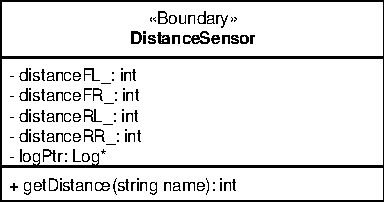
\includegraphics[]{../fig/diagrammer/bil/cd_distancesensor.pdf}
\caption{Klassebeskrivelse af boundary-klassen DistanceSensor}
\label{fig:cd_distancesensor}
\end{figure}

\textbf{Attributter}

\begin{table}[h]
\begin{tabularx}{\textwidth}{| Z | Z | L{10cm} |} \hline
Navn & Type & Beskrivelse \\\hline
\texttt{addrFL} & \texttt{int} &Adresse til forreste venstre afstandssensor.\\\hline
\texttt{addrFR} & \texttt{int} &Adresse til forreste højre afstandssensor.\\\hline
\texttt{addrRL} & \texttt{int} &Adresse til bagerste venstre afstandssensor.\\\hline
\texttt{addrRR} & \texttt{int} &Adresse til bagerste højre afstandssensor.\\\hline
\texttt{distanceFL} & \texttt{int} &Midlertidig variabel der indeholder afstanden fra forreste venstre afstandssensor.\\\hline
\texttt{distanceFR} & \texttt{int} &Midlertidig variabel der indeholder afstanden fra forreste højre afstandssensor.\\\hline
\texttt{distanceRL} & \texttt{int} &Midlertidig variabel der indeholder afstanden fra bagerste venstre afstandssensor.\\\hline
\texttt{distanceRR} & \texttt{int} &Midlertidig variabel der indeholder afstanden fra bagerste højre afstandssensor.\\\hline
\texttt{fd} & \texttt{int} &Variabel der anvendes som reference til i2c-bussen som sensorerne er tilkoblet\\\hline
\texttt{logEntry} & \texttt{string} &Variabel der indeholder reference til loggen.\\\hline
\end{tabularx}
\caption{Attributter for klassen DistanceSensor}
\label{table:attr_distancesensor}
\end{table}

\textbf{Metoder}

\begin{table}[h]
\begin{tabularx}{\textwidth}{| L{2.5 cm} | Z |} \hline
Prototype & \texttt{int getDistance(string name)} \\\hline
Parametre & \texttt{name} \newline Navnet på den sensor som der skal læses fra. Kan en af fire muligheder "FL", "FR", "RL" og "RR". \\\hline
Returværdi &  \texttt{int} \newline Afstanden for til nærmeste sensor for den pågældende sensor. Tallet er angivet i cm. \\\hline
Beskrivelse & Metoden læser afstanden som en afstandssensor befinder sig fra en forhindring. \\\hline
\end{tabularx}
\caption{Metodebeskrivelse for \texttt{getDistance}}
\label{table:met_getdistance}
\end{table}
\clearpage


Afstandssensorene leveres formonteret på chip hvor benene fra IC'en er trukket til harwinpins som let kan tilgås. Til kommunikationen benyttes følgende linjer: 

\begin{itemize}
	\item pin 7: VCC: Forsyning
	\item pin 6: GND: Reference
	\item pin 5: SCL: Clock
	\item pin 4: SDA: Data
	\item pin 3: Benyttes ikke
	\item pin 2: Status
	\item pin 1: Temp adresse 
\end{itemize}

Data kommunikeres på SDA-linjen med reference til clock'en. ''Status'' benyttes til at angive om sensoren er i gang med at performe en ''range reading''. 
Pin'en holdes højt så længe sensoren scanner, og trækkes lavt når operationen er fuldført og data kan leveres. Når pin'en er høj ignoreres al I2C-kommunikation.

For at initiere sensoren, ''Temp-adresse''-pin'en hvor der sendes en unik 7-bit adresse til sensoren.
   
Afstandssensorene benytter sig af I2C-bussen til kommunikation med Pi'en. Hertil benyttes I2C-tools biblioteket.
Dette bibliotek skal derfor hentes og aktiveres i linux-distrubutionen.

I2C device filer er CDD med major-nummer 89, og hver enkelt adaptor der er tilkoblet systemet får vedhæftet et minor-nummer, 
disse device filer findes i /dev/i2c-X, hvor X er et unik minor-nummer fra 0-256. Herfter er hver enkelt i2c-adaptor nu identificerbar og kan tilgås enkeltvis. 

Herefter skrives en klasse der kan håndtere de ønskede kald til de 4 afstandssensorer. 
I dette tilfælde ønskes der at implementere initDistance() og en getDistance() og i disse funktioner benyttes systemkald til at tilgå Hardwaren direkte, og aflæse de 4 sensorer via I2C-bussen.
\clearpage
\subsubsection{Domain-klasse: Data} \label{sec:data_klasse}

Data-klassen indeholder alt den nyeste data, som enten skal sendes til brugerinterfacet eller som kommer fra brugerens input på Xbox-360 controlleren. Klassen har ikke anden reel funktionalitet end at beskytte data'en mod at blive korrupt hvis der er flere tråde der skriver eller læser fra den på en gang. Dette gøres ved hjælp af \texttt{std::mutex}es. Undervejs i implementeringsfasen er dette klasse testet grundigt ved brug af et stort antal tråde som alle forsøger at skrive til- o læse fra datastrukturen på samme tid.
\clearpage
\subsubsection{Domain-klasse: Log}

Loggen har til formål at kunne lokalisere og identificere fejl i systemet. Loggen skal oprettes mere eller mindre globalt og der skal efterfølgende medgives en pointer til samtlige klasser på Pi. Alle disse klasser skal således anvende loggen som debugging redskab. Der skal som udgangspunkt kun skrives i loggen hvis en fejl opstår, da loggen ellers bliver uoverskuelig. Når der skrives til loggen, anvender den pågældende tråd cpu-tid, hvilket ligeledes er en grund til at være opmærksom på hvornår det er smart at skrive til loggen. \\
For at forhindre at log-entries fra forskellige tråde sammenflettes, skal der i implementeringen anvendes \texttt{std::mutex} som lås når der skrives i loggen.

\begin{figure}[h]
\centering
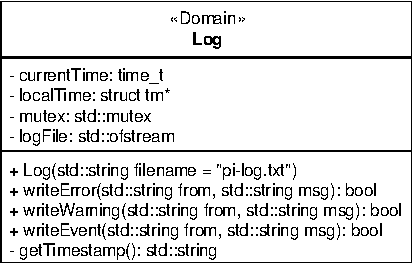
\includegraphics[]{../fig/diagrammer/bil/cd_log.pdf}
\caption{Klassebeskrivelse for domain-klassen Log}
\label{fig:cd_log}
\end{figure}

\textbf{Attributter}

\begin{table}[h]
\begin{tabularx}{\textwidth}{| Z | Z | L{10cm} |} \hline
Navn & Type & Beskrivelse \\\hline

\texttt{currentTime} & \texttt{time\_t} &Denne attribut bruges til at gemme det nuværende tidspunkt, når \texttt{getTimestamp} kaldes. \\\hline

\texttt{localTime} & \texttt{struct tm*} & Anvendes til at holde tiden i et læseligt format. \\\hline

\texttt{mutex} & \texttt{std::mutex} & Anvendes som lås i \texttt{std::lock\_guard} der forhindrer flere tråde i at skrive i loggen på samme tid. \\\hline

\texttt{logFile} & \texttt{std::ofstream} & File descriptor til logfilen. \\\hline

\end{tabularx}
\caption{Attributter for klassen Log}
\label{table:attr_log}
\end{table}


\textbf{Constructor}
%------------------------------------- Log -------------------------------------
\begin{table}[h]
\begin{tabularx}{\textwidth}{| L{2.5 cm} | Z |} \hline
Prototype & \texttt{Log(std::string filename = ''pi-log.txt'')} \\\hline
Parametre & \texttt{filename} \newline Det ønskede filnavn til logfilen der oprettes. Hvis denne parameter udelades ved initialiseringen bliver objektet oprettet med filnavnet ''pi-log.txt''.  \\\hline
Beskrivelse & Constructoren opretter et objekt af Log klassen med det angivne filnavn. \\\hline
\end{tabularx}
\caption{Beskrivelse af constructor for \texttt{Log}}
\label{table:con_log}
\end{table}

\clearpage

\textbf{Metoder}
%------------------------------------- writeError -------------------------------------
\begin{table}[h]
\begin{tabularx}{\textwidth}{| L{2.5 cm} | Z |} \hline
Prototype & \texttt{bool writeError(std::string from, std::string msg)} \\\hline
Parametre & \texttt{from} \newline Denne streng skal udfyldes med den indbyggede identifier ''\texttt{\_\_PRETTY\_FUNCTION\_\_}'' (GNU standard) der returnerer placeringen af det pågældende kald. Herved kan det i loggen ses præcis i hvilken klasse og metode log-beskeden kommer fra. \newline \newline \texttt{msg} \newline Den besked der skal stå i loggen. \\\hline
Returværdi &  \texttt{bool} \newline Returnerer \texttt{true} hvis skrivningen er gået godt og \texttt{false} hvis skrivningen gik galt. \\\hline
Beskrivelse & Metoden skriver en besked i loggen. Anvendes når der er sket en alvorlig fejl. \\\hline
\end{tabularx}
\caption{Metodebeskrivelse for \texttt{writeError}}
\label{table:met_writeError}
\end{table}

%------------------------------------- writeWarning -------------------------------------
\begin{table}[h]
\begin{tabularx}{\textwidth}{| L{2.5 cm} | Z |} \hline
Prototype & \texttt{bool writeWarning(std::string from, std::string msg)} \\\hline
Parametre & \texttt{from} \newline Denne streng skal udfyldes med den indbyggede identifier ''\texttt{\_\_PRETTY\_FUNCTION\_\_}'' (GNU standard) der returnerer placeringen af det pågældende kald. Herved kan det i loggen ses præcis i hvilken klasse og metode log-beskeden kommer fra. \newline \newline \texttt{msg} \newline Den besked der skal stå i loggen. \\\hline
Returværdi &  \texttt{bool} \newline Returnerer \texttt{true} hvis skrivningen er gået godt og \texttt{false} hvis skrivningen gik galt. \\\hline
Beskrivelse & Metoden skriver en besked i loggen. Anvendes når der er sket en mindre alvorlig fejl. \\\hline
\end{tabularx}
\caption{Metodebeskrivelse for \texttt{writeWarning}}
\label{table:met_writeWarning}
\end{table}

\clearpage

%------------------------------------- writeEvent -------------------------------------
\begin{table}[h]
\begin{tabularx}{\textwidth}{| L{2.5 cm} | Z |} \hline
Prototype & \texttt{bool writeEvent(std::string from, std::string msg)} \\\hline
Parametre & \texttt{from} \newline Denne streng skal udfyldes med den indbyggede identifier ''\texttt{\_\_PRETTY\_FUNCTION\_\_}'' (GNU standard) der returnerer placeringen af det pågældende kald. Herved kan det i loggen ses præcis i hvilken klasse og metode log-beskeden kommer fra. \newline \newline \texttt{msg} \newline Den besked der skal stå i loggen. \\\hline
Returværdi &  \texttt{bool} \newline Returnerer \texttt{true} hvis skrivningen er gået godt og \texttt{false} hvis skrivningen gik galt. \\\hline
Beskrivelse & Metoden skriver en besked i loggen. Anvendes når der er hændelse, der ikke er en fejl, som skal skrives i loggen. \\\hline
\end{tabularx}
\caption{Metodebeskrivelse for \texttt{writeEvent}}
\label{table:met_writeEvent}
\end{table}

%------------------------------------- getTimestamp -------------------------------------
\begin{table}[h]
\begin{tabularx}{\textwidth}{| L{2.5 cm} | Z |} \hline
Prototype & \texttt{std::string getTimestamp()} \\\hline
Parametre & ~ \newline \\\hline
Returværdi &  \texttt{std::string} \newline Returnerer en streng med systemets indstillede tid og dato. Formatet er \texttt{ÅÅÅÅ-MM-DD TT:MM:SS}.\\\hline
Beskrivelse & Metoden henter den nuværende tid i systemet og omdanner denne til en streng i en format der nemt kan anvendes i log-beskeder. \\\hline
\end{tabularx}
\caption{Metodebeskrivelse for \texttt{getTimestamp}}
\label{table:met_getTimestamp}
\end{table}
\clearpage
\subsubsection{Domain-klasse: Settings} %TODO lav label

%TODO skal skrives
\clearpage
% ++++++++++++ Domain Pi AKS klassen ++++++++++++++
\subsubsection{Domain-klasse: Aks}\label{sec:aks_design}

\begin{figure}[h]
\centering
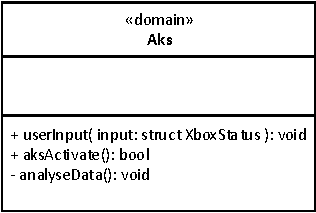
\includegraphics[scale=1]{../fig/diagrammer/bil/cd_aks.pdf}
\caption{Klassebeskrivelse for domain-klassen Aks}
\label{fig:cd_aks}
\end{figure}

\textbf{Attributter}

\begin{table}[h]
\begin{tabularx}{\textwidth}{| Z | Z | L{9cm} |} \hline
Navn & Type & Beskrivelse \\\hline
\texttt{MySteering} & \texttt{Steering} & Styretøjsklassen, bruges når Aks skal påvirke bilens hastighed eller retning.\\\hline
\texttt{MyData} & \texttt{Data*} & Pointer til bilens datastruktur.\\\hline
\texttt{MySettings} & \texttt{Settings*} & Pointer til Settingsklassen. \\\hline
\texttt{MyLog} & \texttt{Log*} & Pointer til loggen. \\\hline
\texttt{state} & \texttt{aksStates} & Husker hvilket stadie bilen er i, kan skifte mellem at stå stille, køre fremad/bagud eller trille. \\\hline
\texttt{proxSensors} & \texttt{int*} & Et array med nuværende værdier fra afstandssensorer \\\hline
\texttt{old\_proxSensors} & \texttt{int*} & Et array der holder de foregående værdier fra afstandssensorer \\\hline
\texttt{latestUserInput} & \texttt{UserInput} & Gemmer de seneste input fra brugeren. \\ \hline
\end{tabularx}
\caption{Attributter for klassen Aks}
\label{table:attr_aks}
\end{table}

\textbf{Metoder}


%----------------- aksActivate -------------------
\begin{table}[h]
\begin{tabularx}{\textwidth}{| L{2.5 cm} | Z |} \hline
Prototype & \texttt{void aksActivate(void)} \\\hline
Parametre & \texttt{void}  \\\hline
Returværdi &  \texttt{bool} \newline Returnerer \texttt{TRUE} hvis det gik godt og \texttt{FALSE} hvis der skete fejl undervejs. \\\hline
Beskrivelse & Metoden kaldes når det automatiske anti-kollisionssystem skal aktiveres. Forhindrer samtidigt input fra brugeren kortvarigt. \\\hline
\end{tabularx}
\caption{Metodebeskrivelse for \texttt{aksActivate}}
\label{table:met_aks_aksActivate}
\end{table}

%----------------- analyseData -------------------
\begin{table}[h]
\begin{tabularx}{\textwidth}{| L{2.5 cm} | Z |} \hline
Prototype & \texttt{void analyseData(void)} \\\hline
Parametre & \texttt{void}  \\\hline
Returværdi &  \texttt{void}  \\\hline
Beskrivelse & Metoden analyserer indhentet data fra Data klassen og vurderer hvilken type af undvigelse der bedst passer. Aktiverer herefter Steering-klassen for at bilen skal undvige forhindringen. \\\hline
\end{tabularx}
\caption{Metodebeskrivelse for \texttt{analyseData}}
\label{table:met_aks_analyseData}
\end{table}
\clearpage
\subsubsection{Boundary-klasse: PcCom} \label{sec:pccom}
PcCom klassens formål er at give mulighed for PC softwaren at skabe kontakt mellem Bil og PC. Den blev som udgangspunkt designet med en UDP protokol, men efter implementering af PC software blev dette skiftet til en TCP protokol, da softwaren var blevet implementeret således. PcCom klassen er designet og implementeret som to tråde der her især åbner en server med TCP sockets til at styre to forskellige former for datastreams mellem Bil og PC. Trådene er implementeret ved brug af biblioteket \texttt{thread}, som giver anledning til konstruktion af et object af typen \texttt{std::thread}. Disse objekter er tråde der hver især er en sekvens af instruktioner, der kan udføres sammen med andre sådanne sekvenser i multithreading miljøer. Der er under design og implementering ligeledes draget meget nytte af ''Sockets Tutorial'' \cite{lib:socket_tutorial}, en instruktion i at implemntere TCP scokets på en linux maskine.
\clearpage
\subsection{Steeringklassen} \label{sec:steering_impl}

Steering klassen er den klasse der kontrollere PWM signalet til motorens fremdrift og til styretøj servoen. 
Den modtager nye input fra systemet om ændringer af fremdrift, retning på styretøj og brems. Derudover henter den, hver gang klassen skal opdaterer PWM signalet til motoren, den aktuelle hastighed på bilen fra Dataklassen. 
Klassen har kun en public metode den kan kaldes. I listing \ref{lst:steering_header} ses implementering af klassens headerfilen.\newline

\lstinputlisting[linerange=Steering::header1-Steering::header2, label=lst:steering_header, caption=\texttt{Header} for Steeringklassen.]{../../src/bil/steering/steering.hpp}

Constructoen sørger primært for at sætte WiringPi op. Se sektion \ref{sec:wiringPi_impl}. 
Der er en HW og SW PWM del der skal initialiseres. 
Udover opsætning starter den en separat tråd der kører \texttt{PWMUpdate} i et loop indtil systemet lukkes ned. 
Samt at sætte værdier for PID regulering af motoren 

\lstinputlisting[linerange=Steering::Steering1-Steering::Steering2, label=lst:steering_con, caption=\texttt{Constructor} for Steeringklassen.]{../../src/bil/steering/steering.cpp}


Deconstructoen sørger for at lukke \texttt{Steering::PWMUpdate} tråden ned og joine med den, slukke for HW og SW PWM og digitale outputs til styring af H-broen.

\lstinputlisting[linerange=Steering::~Steering1-Steering::~Steering2, label=lst:steering_decon, caption=\texttt{Deconstructor} for Steeringklassen.]{../../src/bil/steering/steering.cpp}

Metoden \texttt{userInput} er den eneste metode der kan tilgås udefra. Den håndtere værdier fra Xbox 360 kontrolleren. Den omregner frem og tilbage værdierne i forhold den max hastighed der er sat for bilen. Max hastigheden hentes fra Settings klassen. Hvis der skal bremses går den direkte til \texttt{brake} metoden. Tilsidst kalder \texttt{turn} metoden

\lstinputlisting[linerange=Steering::userInput1-Steering::userInput2, label=lst:steering_userInput, caption=Metoden \texttt{userInput} Steeringklassen.]{../../src/bil/steering/steering.cpp} 

\texttt{brake} metoden bremser bilen ved at sætte motor PWM til 100 \% og de 2 retnings digitale outputs lave. Det får H-broen til at bremse motoren aktivt. Mens der bremses bliver PWM i \texttt{PWMUpdate} ikke opdateret.
\lstinputlisting[linerange=Steering::brake1-Steering::brake2, label=lst:steering_brake, caption=Metoden \texttt{brake} Steeringklassen.]{../../src/bil/steering/steering.cpp}

\texttt{softbrake} metoden sætte motor PWM til 0 \% og de 2 retnings digitale outputs lave. 
Derved vil bilen begynde at løbe farten af.
\lstinputlisting[linerange=Steering::softbrake1-Steering::softbrake2, label=lst:steering_softbrake, caption=Metoden \texttt{softbrake} Steeringklassen.]{../../src/bil/steering/steering.cpp}

\texttt{turn} metoden omregner styre værdierne fra Xbox kontrolleren til en duty cycle for SW PWM mellem 0,5ms og 2.5ms. 
Som vil give max udslag til begge sider. 
\lstinputlisting[linerange=Steering::turn1-Steering::turn2, label=lst:steering_turn, caption=Metoden \texttt{turn} Steeringklassen.]{../../src/bil/steering/steering.cpp}

\texttt{motorSetPWM} metoden bestemmer om bilen skal sættes til at kører frem eller tilbage ud fra den aktuelle retning og input fra Xbox kontrolleren. 
Hvis det er nødvendig at kører den modsatte vej bremses der indtil den er under en vis hastighed
. 
\lstinputlisting[linerange=Steering::motorSetPWM1-Steering::motorSetPWM2, label=lst:steering_motorSetPWM, caption=Metoden \texttt{motorSetPWM} Steeringklassen.]{../../src/bil/steering/steering.cpp}

\texttt{PWMUpdate} metoden kører i sin egen tråd. Den henter hver gang den aktuelle hastighed på bilen fra \texttt{Dataklassen} og udregner fejlen i forhold til den ønskede hastighed. Herefter udregner værdierne for PID reguleringen. Og til sidst sættes den nye PWM værdi på motoren. 
\lstinputlisting[linerange=Steering::PWMUpdate1-Steering::PWMUpdate2, label=lst:steering_PWMUpdate, caption=Metoden \texttt{PWMUpdate} Steeringklassen.]{../../src/bil/steering/steering.cpp}

\subsubsection{Test af Steering klassen}


\lstinputlisting[linerange=main::main1-main::main2, label=lst:steering_main, caption=Test af \texttt{Steering klassen} Steeringklassen.]{../../src/bil/steering/main.cpp}

\subsubsection*{WiringPi} \label{sec:wiringPi_impl}